\chapter{Related Work}
\label{ch:relatedwork}

This chapter will introduce several preexisting technologies in the different areas that my tool will be focusing on. These areas are the automatic installation of Docker on a given machine, a graphical user interface for the interaction with different elements of Docker, and finally, a tool which upon being supplied with a file path to a directory will write a Dockerfile that can run any programs in that directory. It will then perform an analysis of these different components and illustrate what aspects I will be mimicking in the final tool and what elements I will improve upon.

\break

\section{Docker Installer}
\label{sec:installer}

There are several preexisting tools for automatically installing Docker onto a machine. These tools are Docker Desktop and Docker Toolbox. There are several issues with these installers. The first issue is that these installers are only for Mac OS and Windows, meaning that there is currently not an official Docker installer for Linux. These tools can be found on Docker's official website along with installation instructions and a lot more information on which someone who is just starting to learn how to use Docker, will not need it. The sheer amount of information that is present can also make figuring out what the correct installer is difficult.

This can be seen in the documented steps for installing Docker on Linux distributions which alone have five different pages for the various distributions of Linux and an additional sixth page for optional post-installation instructions \cite{dockerDocs}.

However, the biggest installation issue comes when a user tries to install Docker on Windows as there are two distinct versions of Docker for Windows, Docker Desktop for Windows Professional users and Docker Toolbox for Windows Home users. Unfortunately, both of these versions require the user to turn on Virtualization technology, which can only be done from the BIOS settings. The next issue with the Windows version comes in the form of the actual installer that is provided by Docker. This installer will sometimes install incorrect or versions of required software that are known to be buggy, mainly a version of VirtualBox is a Software tool for creating Virtual Machines and is required to use Docker on Windows.

In contrast to Windows Home, which uses the Docker Toolbox, Windows Professional uses a program called Docker Desktop, which in my experience has a much higher first-time installation success rate. The reason for this the difference in version comes down strictly to a minor difference between Windows Home and Windows Professional. This difference is the installation of Hyper-V technology, something which Microsoft allows to be installed on Windows Professional but not Windows Home, thus requiring Home users to install Docker Toolbox.

Mac OS users have it much easier as there is only a single install for the operating system which when run will install Docker correctly. There is the bonus of Mac OS being a Unix based system so if a user installs Homebrew, they can use the command line to interact with Docker and not have to rely on graphical interfaces if they prefer to use the command line.

\section{Docker Interface}
\label{sec:interface}

There are currently several graphical interfaces available for the creation and management of Docker containers. One of these interfaces comes directly from Docker and is known as Kitematic \cite{kitematic}, which has the added advantage of being officially supported by the developers of Docker. This will allow for Kitematic to stay up to date with any changes that Docker may make and in theory, would allow it to be the best interface This program, however, is only available for Mac OS and Windows and will not run on Linux distributions. Looking at the interface itself, however, illustrates the amount of time that Docker Inc. has placed into making sure that the interface is usable. This is because the interface is overall very simple and clean looking, there is not a lot of extraneous text or options and it allows for a user to easily download an image from Docker Hub and have a container running. From there Kitematic also includes an in interface terminal for interaction with containers which allows for Kitematic to be a 'one-stop-shop' for Docker users. However, while this may make using Docker easier for anyone to use it does not necessarily allow for a user to learn the backend aspects of building and running an image and/or a container.

\begin{figure}[h!]
    \centering
    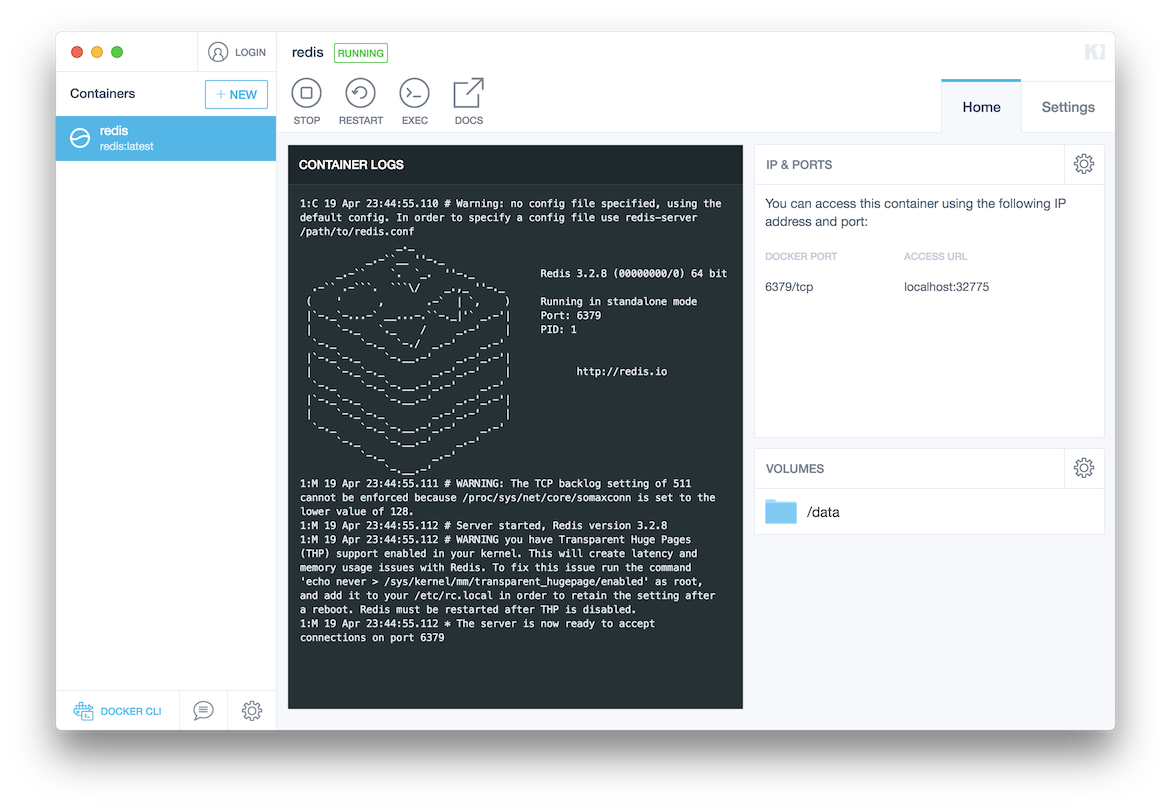
\includegraphics[width=5in]{images/Kitematic}
    \caption{Kitematic Dashboard}
\end{figure}

The main limitations of Kitematic, not supporting all operating systems, are not found in other interfaces like DockStation, which supports Linux as well as Mac OS and Windows. However, DockStation \cite{dockstation} does not install any form of Docker along with itself and as such requires a successful installation before it can be utilized. Another limitation of DockStation is that it requires the use of Docker Compose, which is an additional installation which is not included in the base Docker for Linux. An additional limitation of DockStation is it does not allow for the running of Docker images, only Docker containers. This, in turn, does not allow for a user to use the '--rm' command line flag when running an image that deletes the resulting container upon exiting the container. Dockstation also has additional tools that allow for the monitoring of local and remote Docker containers and other utilities that are aimed more at higher level users of Docker. Among the information provided is the current status of the container as well as all logs that are created in the process of it running.

\begin{figure}[h!]
    \centering
    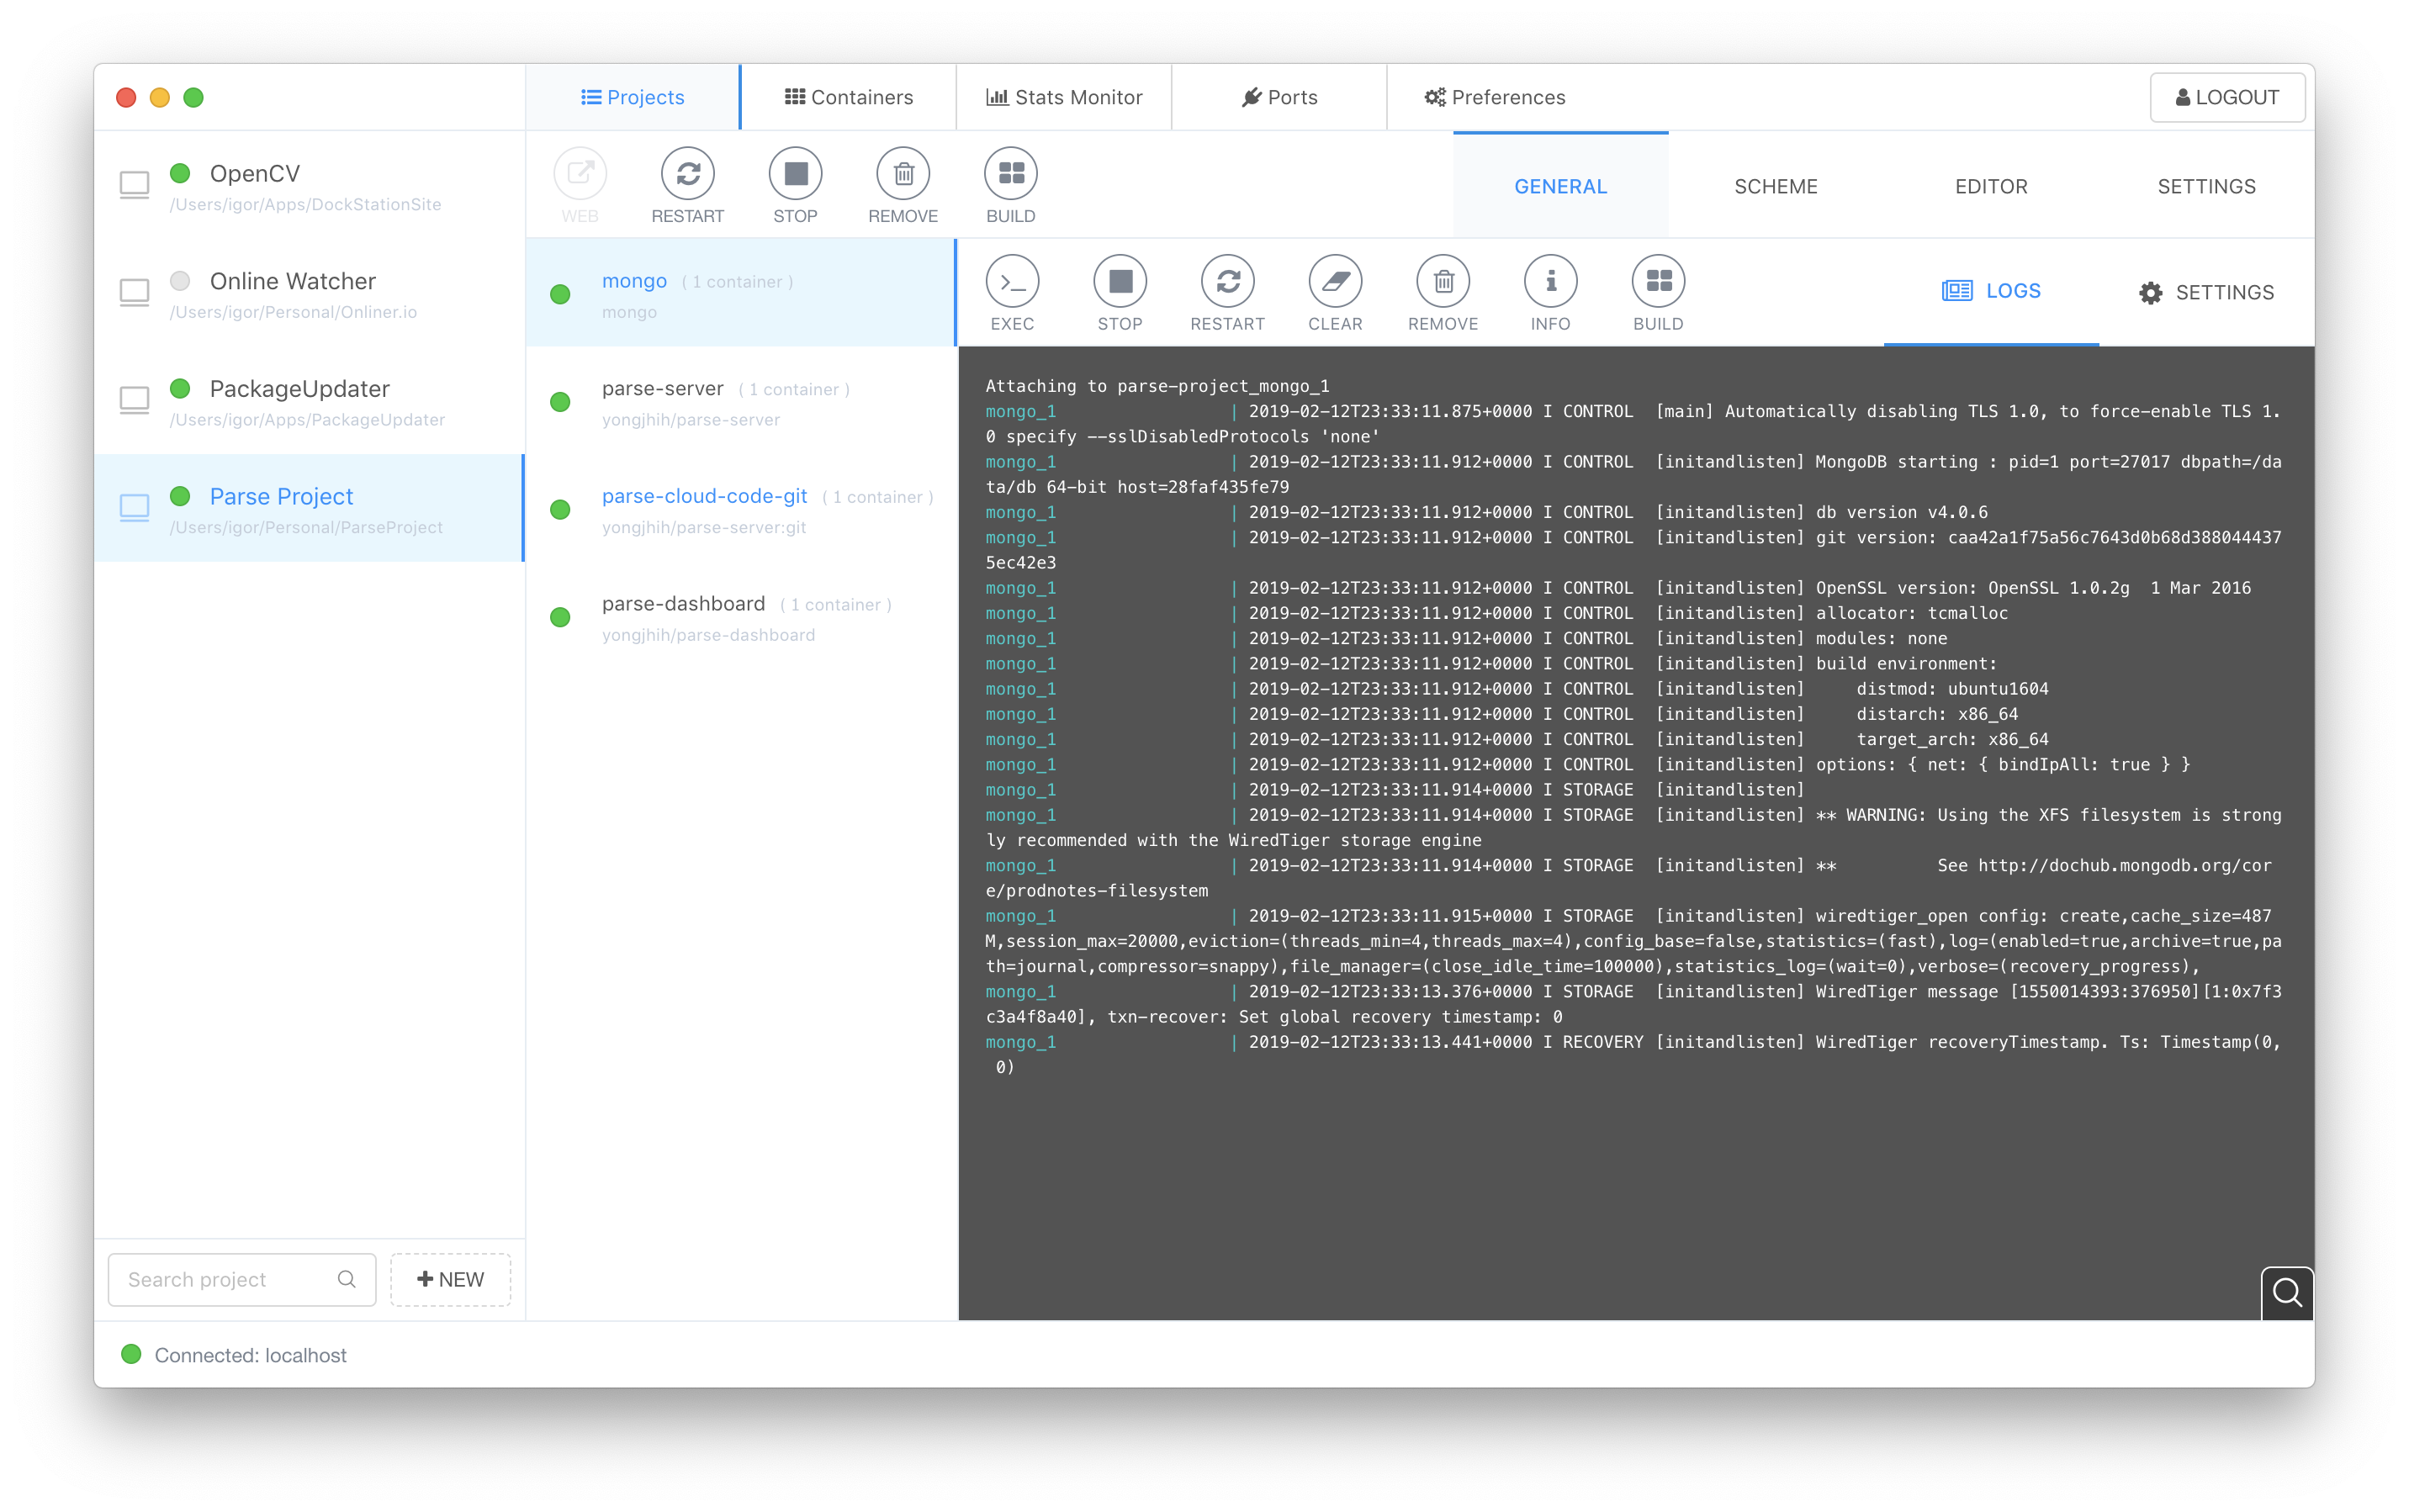
\includegraphics[width=5in]{images/DockStation}
    \caption{DockStation Interface}
\end{figure}

A graphical interface that works well and looks good is Portainer \cite{portainer}, this interface is a web-based application and allows for the creation and running of images and containers. However, the largest limitation with Portainer is that it requires Docker for it to be run and does not install Docker alongside itself like Kitematic. Portainer also has many features that DockStation does, like the remote monitoring of containers that are running and a system for easily creating containers quickly and easily. Despite requiring Docker to run, Portainer has a very intuitive interface that I will base my interface on. The simplistic nature of the overall tool makes it easy to figure out. It also is a rather lightweight application and only requires enough memory to run due to it running inside of a Docker container. However, I will not include some of the elements that I deem to be not needed or even redundant like networks, which for an introductory level Docker interface is not necessary.

\begin{figure}[h!]
    \centering
    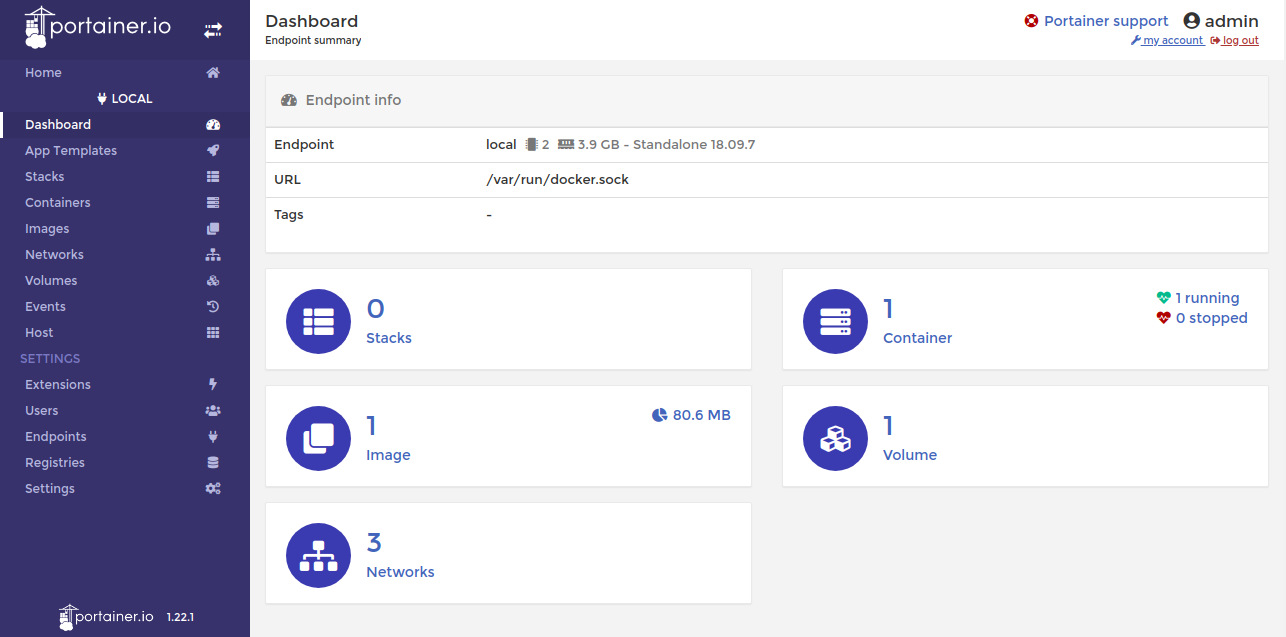
\includegraphics[width=5in]{images/Portainer}
    \caption{Portainer Dashboard}
\end{figure}

\section{Dockerfile Generator}
\label{sec:generator}

Tools that help the user to generate a Dockerfile are not very common due to the sheer number of ways that a Dockerfile can be written to accomplish the same task. However, in my search, I was able to find a single tool that had similarities to what I hope to accomplish, Microsoft's Generator-docker for Linux terminals \cite{microsoft_2018}. This tool, which was written in JavaScript allows for a user to specify the language of the project that they want to be run in the container along with several other factors, like the name of the image and the port, the application will be listening to.

However, this tool has many limitations. The first limitation is that the process is not automatic, the user has to specify the language that the container will use and there can only be a single language specified. Along the lines of programming language, this tool only supports three languages, .NET Core, Node.js, and Golang, which does allow for a closer degree of customization of the Dockerfile but does create a limitation in the number of projects that would be supported. This aspect is something that will, hopefully, not be a part of the generator tool that I create.

This tool, on the other hand, does have features that will be a part of or similar to features in the final Dockerfile generator which I create. The main feature which will be present is a way for a user to build and run their Docker image after the creation of the Dockerfile. This feature will not necessarily be a part of the generator and will instead be a feature of the graphical interface. With Generator-docker this code is contained and ran by a separate program written in bash that is automatically generated by the generator. Where my tool will differ from this approach is instead of creating a separate program that can be used to build and run the image, the graphical interface will have the option to build the image as well as to run a specified image.

\section{Overall Tool}
\label{sec:overall}

There are currently no tools available which combine all three aspects of the tool that I will be creating. A slight exception to this is the interface Kitematic which was mentioned in the Interface section \ref{sec:interface}. This is an interface, as previously mentioned, that has been developed by Docker and as such Kitematic is included with Docker Toolbox and Docker Desktop. However, due to this fact if a user faces any issues when trying to install Docker then the inclusion of the Kitematic interface is useless. Due to the lack of all in one tool in this overall area of Docker tools the development of the tool that I will be creating will greatly benefit the Docker community.
